% Options for packages loaded elsewhere
\PassOptionsToPackage{unicode}{hyperref}
\PassOptionsToPackage{hyphens}{url}
%
\documentclass[
  man,floatsintext]{apa6}
\usepackage{amsmath,amssymb}
\usepackage{lmodern}
\usepackage{iftex}
\ifPDFTeX
  \usepackage[T1]{fontenc}
  \usepackage[utf8]{inputenc}
  \usepackage{textcomp} % provide euro and other symbols
\else % if luatex or xetex
  \usepackage{unicode-math}
  \defaultfontfeatures{Scale=MatchLowercase}
  \defaultfontfeatures[\rmfamily]{Ligatures=TeX,Scale=1}
\fi
% Use upquote if available, for straight quotes in verbatim environments
\IfFileExists{upquote.sty}{\usepackage{upquote}}{}
\IfFileExists{microtype.sty}{% use microtype if available
  \usepackage[]{microtype}
  \UseMicrotypeSet[protrusion]{basicmath} % disable protrusion for tt fonts
}{}
\makeatletter
\@ifundefined{KOMAClassName}{% if non-KOMA class
  \IfFileExists{parskip.sty}{%
    \usepackage{parskip}
  }{% else
    \setlength{\parindent}{0pt}
    \setlength{\parskip}{6pt plus 2pt minus 1pt}}
}{% if KOMA class
  \KOMAoptions{parskip=half}}
\makeatother
\usepackage{xcolor}
\usepackage{longtable,booktabs,array}
\usepackage{calc} % for calculating minipage widths
% Correct order of tables after \paragraph or \subparagraph
\usepackage{etoolbox}
\makeatletter
\patchcmd\longtable{\par}{\if@noskipsec\mbox{}\fi\par}{}{}
\makeatother
% Allow footnotes in longtable head/foot
\IfFileExists{footnotehyper.sty}{\usepackage{footnotehyper}}{\usepackage{footnote}}
\makesavenoteenv{longtable}
\usepackage{graphicx}
\makeatletter
\def\maxwidth{\ifdim\Gin@nat@width>\linewidth\linewidth\else\Gin@nat@width\fi}
\def\maxheight{\ifdim\Gin@nat@height>\textheight\textheight\else\Gin@nat@height\fi}
\makeatother
% Scale images if necessary, so that they will not overflow the page
% margins by default, and it is still possible to overwrite the defaults
% using explicit options in \includegraphics[width, height, ...]{}
\setkeys{Gin}{width=\maxwidth,height=\maxheight,keepaspectratio}
% Set default figure placement to htbp
\makeatletter
\def\fps@figure{htbp}
\makeatother
\setlength{\emergencystretch}{3em} % prevent overfull lines
\providecommand{\tightlist}{%
  \setlength{\itemsep}{0pt}\setlength{\parskip}{0pt}}
\setcounter{secnumdepth}{-\maxdimen} % remove section numbering
% Make \paragraph and \subparagraph free-standing
\ifx\paragraph\undefined\else
  \let\oldparagraph\paragraph
  \renewcommand{\paragraph}[1]{\oldparagraph{#1}\mbox{}}
\fi
\ifx\subparagraph\undefined\else
  \let\oldsubparagraph\subparagraph
  \renewcommand{\subparagraph}[1]{\oldsubparagraph{#1}\mbox{}}
\fi
\newlength{\cslhangindent}
\setlength{\cslhangindent}{1.5em}
\newlength{\csllabelwidth}
\setlength{\csllabelwidth}{3em}
\newlength{\cslentryspacingunit} % times entry-spacing
\setlength{\cslentryspacingunit}{\parskip}
\newenvironment{CSLReferences}[2] % #1 hanging-ident, #2 entry spacing
 {% don't indent paragraphs
  \setlength{\parindent}{0pt}
  % turn on hanging indent if param 1 is 1
  \ifodd #1
  \let\oldpar\par
  \def\par{\hangindent=\cslhangindent\oldpar}
  \fi
  % set entry spacing
  \setlength{\parskip}{#2\cslentryspacingunit}
 }%
 {}
\usepackage{calc}
\newcommand{\CSLBlock}[1]{#1\hfill\break}
\newcommand{\CSLLeftMargin}[1]{\parbox[t]{\csllabelwidth}{#1}}
\newcommand{\CSLRightInline}[1]{\parbox[t]{\linewidth - \csllabelwidth}{#1}\break}
\newcommand{\CSLIndent}[1]{\hspace{\cslhangindent}#1}
\ifLuaTeX
\usepackage[bidi=basic]{babel}
\else
\usepackage[bidi=default]{babel}
\fi
\babelprovide[main,import]{english}
% get rid of language-specific shorthands (see #6817):
\let\LanguageShortHands\languageshorthands
\def\languageshorthands#1{}
% Manuscript styling
\usepackage{upgreek}
\captionsetup{font=singlespacing,justification=justified}

% Table formatting
\usepackage{longtable}
\usepackage{lscape}
% \usepackage[counterclockwise]{rotating}   % Landscape page setup for large tables
\usepackage{multirow}		% Table styling
\usepackage{tabularx}		% Control Column width
\usepackage[flushleft]{threeparttable}	% Allows for three part tables with a specified notes section
\usepackage{threeparttablex}            % Lets threeparttable work with longtable

% Create new environments so endfloat can handle them
% \newenvironment{ltable}
%   {\begin{landscape}\centering\begin{threeparttable}}
%   {\end{threeparttable}\end{landscape}}
\newenvironment{lltable}{\begin{landscape}\centering\begin{ThreePartTable}}{\end{ThreePartTable}\end{landscape}}

% Enables adjusting longtable caption width to table width
% Solution found at http://golatex.de/longtable-mit-caption-so-breit-wie-die-tabelle-t15767.html
\makeatletter
\newcommand\LastLTentrywidth{1em}
\newlength\longtablewidth
\setlength{\longtablewidth}{1in}
\newcommand{\getlongtablewidth}{\begingroup \ifcsname LT@\roman{LT@tables}\endcsname \global\longtablewidth=0pt \renewcommand{\LT@entry}[2]{\global\advance\longtablewidth by ##2\relax\gdef\LastLTentrywidth{##2}}\@nameuse{LT@\roman{LT@tables}} \fi \endgroup}

% \setlength{\parindent}{0.5in}
% \setlength{\parskip}{0pt plus 0pt minus 0pt}

% Overwrite redefinition of paragraph and subparagraph by the default LaTeX template
% See https://github.com/crsh/papaja/issues/292
\makeatletter
\renewcommand{\paragraph}{\@startsection{paragraph}{4}{\parindent}%
  {0\baselineskip \@plus 0.2ex \@minus 0.2ex}%
  {-1em}%
  {\normalfont\normalsize\bfseries\itshape\typesectitle}}

\renewcommand{\subparagraph}[1]{\@startsection{subparagraph}{5}{1em}%
  {0\baselineskip \@plus 0.2ex \@minus 0.2ex}%
  {-\z@\relax}%
  {\normalfont\normalsize\itshape\hspace{\parindent}{#1}\textit{\addperi}}{\relax}}
\makeatother

\makeatletter
\usepackage{etoolbox}
\patchcmd{\maketitle}
  {\section{\normalfont\normalsize\abstractname}}
  {\section*{\normalfont\normalsize\abstractname}}
  {}{\typeout{Failed to patch abstract.}}
\patchcmd{\maketitle}
  {\section{\protect\normalfont{\@title}}}
  {\section*{\protect\normalfont{\@title}}}
  {}{\typeout{Failed to patch title.}}
\makeatother

\usepackage{xpatch}
\makeatletter
\xapptocmd\appendix
  {\xapptocmd\section
    {\addcontentsline{toc}{section}{\appendixname\ifoneappendix\else~\theappendix\fi\\: #1}}
    {}{\InnerPatchFailed}%
  }
{}{\PatchFailed}
\usepackage{lineno}

\linenumbers
\usepackage{csquotes}
\ifLuaTeX
  \usepackage{selnolig}  % disable illegal ligatures
\fi
\IfFileExists{bookmark.sty}{\usepackage{bookmark}}{\usepackage{hyperref}}
\IfFileExists{xurl.sty}{\usepackage{xurl}}{} % add URL line breaks if available
\urlstyle{same} % disable monospaced font for URLs
\hypersetup{
  pdftitle={Untitled},
  pdfauthor={Erin Campbell1, Charles P. Davis2, \& Naomi Caselli1},
  pdflang={en-EN},
  hidelinks,
  pdfcreator={LaTeX via pandoc}}

\title{Untitled}
\author{Erin Campbell\textsuperscript{1}, Charles P. Davis\textsuperscript{2}, \& Naomi Caselli\textsuperscript{1}}
\date{}


\shorttitle{Crossling Abstractness}

\authornote{

Correspondence concerning this article should be addressed to Erin Campbell, 2 Silber Way, Boston, MA xxxxx. E-mail: \href{mailto:eecamp@bu.edu}{\nolinkurl{eecamp@bu.edu}}

}

\affiliation{\vspace{0.5cm}\textsuperscript{2} Department of Psychology \& Neuroscience, Duke University, Durham, NC\\\textsuperscript{1} Wheelock College of Education \& Human Development, Boston University, Boston, MA}

\begin{document}
\maketitle

\begin{verbatim}
## Warning: package 'readr' was built under R version 4.0.5
\end{verbatim}

\begin{verbatim}
## Warning: package 'glue' was built under R version 4.0.5
\end{verbatim}

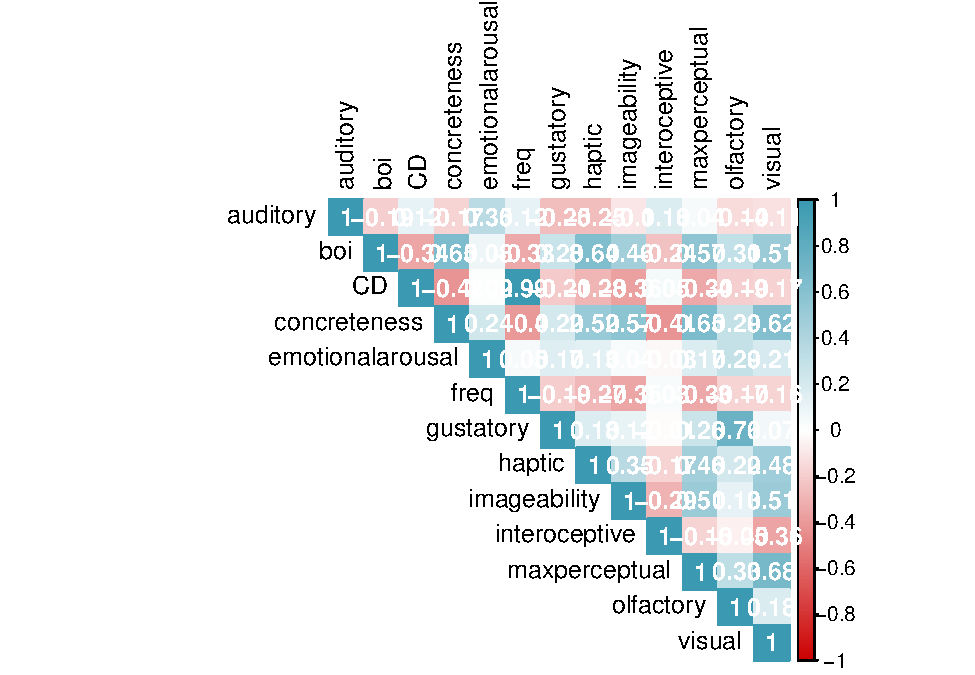
\includegraphics{crossling_abstractness_manuscript_files/figure-latex/source-and-load-1.pdf} 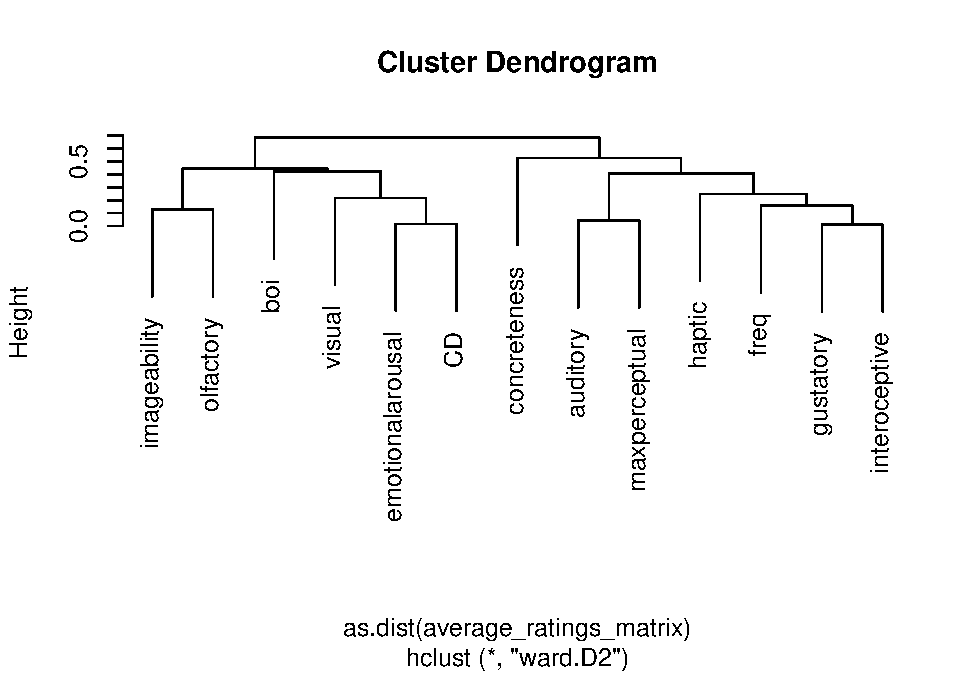
\includegraphics{crossling_abstractness_manuscript_files/figure-latex/source-and-load-2.pdf}

\hypertarget{abstract}{%
\section{Abstract}\label{abstract}}

of vocabulary data from 87507 children

\hypertarget{where-to-send-this}{%
\section{where to send this?}\label{where-to-send-this}}

Open Mind, CogSci (the journal, not the conference), Cognition, DevSci, Language and Cognition

\hypertarget{introduction}{%
\section{Introduction}\label{introduction}}

Young children rapidly learn new words, but some words are easier to learn than others. There are many reasons why a word might be challenging to learn---it is hard to pronounce (e.g., ``sixth''), it is syntactically complex (e.g., ``inedible''), or it is relative abstract, i.e., its referent is not readily observable in the environment (e.g., ``problem''). Here we focus on abstractness as a predictor of when words are learned. Why might words referring to abstract things be challenging to learn? Consider this: you are attempting to teach alien visitors some important words. What properties of words might make your job relatively easy or difficult? Words like ``snake'' would be easy to teach---snakes have a readily identifiable shape and make characteristic sounds---they are strongly associated with particular sensory and perceptual experiences (Lynott, Connell, Brysbaert, Brand, \& Carney, 2020)---and while they vary in size and color, these differences aren't terribly important in determining whether something is a snake or not (whether it is dangerous is another question entirely). Words like ``moo'' might also be readily teachable, as the motivated mapping between the sound of the word and the sound it refers to eases the learning process (e.g., {[}imai2013{]}. Finally, {[}some example illustrating the ``Abstract from specific circumstance'' bit{]} \ldots{}

Each of these three examples highlights different ways we might conceive of abstractness: abstract words can be characterized by an absence of sensory and perceptual features (e.g., want; (\textbf{paivio1971?}; \textbf{paivio1991?})), they may have a less stable mapping between word form and meaning (though cf.~CITE), and they tend to be applicable in a wide range of linguistic contexts (e.g., problem, (\textbf{schwanenflugel1983?}; \textbf{hoffman2013?}; \textbf{davis2020?})). However, research on word learning has typically collapsed these construals into the more general problem of abstract words lacking a stable referent. In the following, we unpack existing research on acquisition of abstract (vs.~concrete) words, before elaborating on each of the proposed construals of abstractness and how each construal might make unique predictions about the effects of abstractness on word learning.

\hypertarget{abstractness-in-acquisition}{%
\subsection{Abstractness in Acquisition}\label{abstractness-in-acquisition}}

children learn abstract words later (\textbf{bergelson2013?})

\hypertarget{different-constructions-of-abstractness}{%
\subsection{Different Constructions of Abstractness}\label{different-constructions-of-abstractness}}

The most oft-cited reason why children tend to acquire abstract words later than concrete ones is because abstract words lack a clear sensory-perceptual referent, and thus are characterized by referential uncertainty (\textbf{bergelson2013?}). However, this explanation rests on a negative definition of abstract words---namely, whereas concrete words refer to things that can be experienced directly through the senses, abstract words refer to things that cannot, and must be instead defined by other words (Brysbaert, Warriner, \& Kuperman, 2014). This view on abstract words is increasingly coming into question, with a growing literature pointing to the richness of experiences associated with abstract words, emphasizing not only that understanding abstract words tends to rely more on language associations (\textbf{paivio1991?}; \textbf{borghi2019?}) and that they tend to be more ambiguous and deployed in diverse lexical and situational contexts (\textbf{schwanenflugel1983?}; \textbf{hoffman2013?}; \textbf{davis2020?}; \textbf{barsalou2018?}) but also that they tend to be highly associated with emotional experience (\textbf{vigliocco2013?}) and social knowledge (\textbf{wilson-mendenhall2013?}). There are also differences between abstract and concrete words in iconicity (i.e., the degree to which a word's meaning is reflected in its form (J. A. Hinojosa, Haro, Magallares, Duñabeitia, \& Ferré, 2021; \textbf{winter2023?}), such that abstract words counterintuitively tend to be rated as more iconic. Assuming a multidimensional perspective on abstract words---that is, that they have a range of experiential properties beyond just a lack of sensory referents---allows us to unpack what properties of abstractness lead to differences in word learning. In the following sections, we consider three different ways in which a word meaning might be abstract: a lack of associated perceptual experience, arbitrary mappings between word form and meaning, and the ability to use a word in a variety of distinct contexts.

\hypertarget{word-meaning-abstract-from-perceptual-experience}{%
\subsubsection{Word Meaning Abstract from Perceptual Experience}\label{word-meaning-abstract-from-perceptual-experience}}

Embodied theories propose that sensorimotor processes are essential for learning the meanings of words (e.g., CITE). Under such hypotheses, words with referents that afford greater sensorimotor experience should be easier to acquire. Greater sensorimotor experience can be thought of both in terms of the saliency of the experience and in terms of the multisensoriness of the experience. English-speaking sighted children, but not blind children, were more likely to produce words when the words are more strongly associated with visual experience (\textbf{campbell2023?}). Seidl, Indarjit, and Borovsky (2023) observed that English words tend to be learned earlier when their semantic associations span multiple senses. In related experimental work, Seidl et al. (2023) observed that 2-year-olds learn words more readily when they are able to interact with the referents than when they are only able to see the referents.

\hypertarget{imageability}{%
\paragraph{Imageability}\label{imageability}}

The property of being something perceptible has traditionally been quantified using two closely related measures: imageability and concreteness. Imageability seeks to capture to what extent a word gives rise to a mental image (\textbf{paivio1968?}), whereas concreteness seeks to identify the degree to which a word is associated with any of the senses, reflecting the totality of subjective sensory experience with a word (Brysbaert et al., 2014). Imageability and concreteness correlate strongly with one another (Rofes et al., 2018), and while they are often used interchangeably, these two constructs tend to diverge based on frequency (e.g., chair and protuberance are similarly concrete, but protuberance is more challenging to summon a mental image for) and specificity (e.g., chair and furniture are similarly imageable, but the more specific word ``chair'' is rated as more concrete). Like concreteness, words rated higher in imageability tend to be processed more quickly {[}cite cite{]} and learned earlier {[}cite cite cite{]}. {[}describe the possible mechanism{]}

\hypertarget{perceptual-strength-and-perceptual-exclusivity}{%
\paragraph{Perceptual Strength and Perceptual Exclusivity}\label{perceptual-strength-and-perceptual-exclusivity}}

More recently, researchers have developed more specific measures of words' perceptual associations. Beyond general perceptibility, these norms separate associations by modality (visual, tactile, auditory, haptic, gustatory, interoceptive), yielding the modality specific ratings, an overall strength rating, and a measure of the spread of ratings across modalities (Lynott et al., 2020). Such specificity allows researchers to test whether information from certain senses, like vision or touch, may be privileged over others {[}cite{]}, as well as whether receiving sensory information from multiple modalities may support acquisition (e.g., Seidl et al. (2023)).

\hypertarget{boi}{%
\paragraph{BOI}\label{boi}}

In English, body-object-interaction ratings predict words' AoA (\textbf{thill2016?}; \textbf{pexman2019?}) and children's lexical processing (\textbf{suggate2017?}; \textbf{wellsby2014?}; \textbf{inkster2016?}), such that words with high sensorimotor interaction ratings are acquired earlier and processed faster. The motor aspect of this relationship may offer additional explanatory power beyond the sensory association effects described in previous paragraphs: the processing speed of high body-object-interaction words (but not low-BOI words) is linked to children's fine motor skills (\textbf{suggate2017?}). Work with adults finds that pairing novel words with motor actions related to their meaning improves learning (\textbf{casasanto2019?}; \textbf{vukovic2019?}), and that activation of the motor cortex is involved in the acquisition of novel words {[}(\textbf{luizzi2010?}); vukovic2019{]}. This effect may be particularly subject to cross-linguistic variation, given the wide cross-cultural variation in infant's motor development (\textbf{cintas2009?}; \textbf{lohaus2014?}).

\hypertarget{word-form-abstract-from-word-meaning}{%
\subsubsection{Word Form Abstract from Word Meaning}\label{word-form-abstract-from-word-meaning}}

Arbitrariness to be a requisite property of language. Language is language because words are abstract symbols of their meaning. Words with an iconic (or motivated) mapping between form and meaning have originally been relegated to the fringes of linguistic discussion. Work on onomatopoeias, ideophones, and systematicity show that iconicity is a more prevalent phenomenon than previously recognized. Across languages, words that are higher in iconicity tend to be learned earlier {[}cite{]}. Some speculate that this is due to easier mapping between the referent and the wordform. Others, however, find this explanation unsatisfying: do young children, who have limited experience, have the world knowledge necessary to recognize these perceptual mappings? It could be that effects of iconicity on acquisition are related to phonological constraints on the meaning of highly-iconic words: highly-iconic words are likely to be concrete {[}cite{]} and carry perceptual information that aligns with the modality of the language (e.g., iconic spoken language words often pertain to auditory referents; iconic sign language words often depict auditory or tactile information; cite)

\hypertarget{word-meaning-abstract-from-specific-circumstance}{%
\subsubsection{Word Meaning Abstract from Specific Circumstance}\label{word-meaning-abstract-from-specific-circumstance}}

\hypertarget{context-diversity-availability}{%
\paragraph{Context Diversity / Availability}\label{context-diversity-availability}}

The diversity of contexts a word appears in predicts word learning in both children (Hills, Maouene, Riordan, \& Smith, 2010; Kachergis, Yu, \& Shiffrin, 2009; Rosa, Salom, \& Perea, 2022) and adults (\textbf{johns2015?}). These effects have been interpreted in line with two processes in early word learning: the lure of the associates, which suggests that words learned earlier tend to be better connected with a range of other known words; and preferential acquisition, where words learned earlier tend to be used in a range of distinct contexts (Hills et al., 2010). The direction of these context diversity effects are variable; in some contexts, verbs(?), are more likely to be learned when the context is more consistent, whereas nouns(?) with diverse contexts are more likely to be learned. More contextually diverse words also tend to be more abstract (\textbf{hoffman2013?}), as abstract words like \emph{idea} have more flexible meanings that can be deployed in a range of contexts, as compared to concrete words like \emph{spaceship}.

Multiple theories: preferential attachment--A word is more likely to enter the lexicon the more connected the known words to which it is related. more highly connected words at Time 1 are more likely to receive new links at Time 2. preferential acquisition---words enter the lexicon not because they are related to well-connected words, but because they connect well to other words in the learning environment (Hills, Maouene, Maouene, Sheya, \& Smith, 2009). Early-learned words may tend to be highly connected because words with greater connectivity in the learning environment are more noticeable and readily learned; that is, children may learn first the most well-connected words in the speech stream to which they are exposed. This is possible because the adult semantic network is both a product of learning and the input (the material to be learned) for the next generation of learners. We call this hypothesis preferential acquisition. lure of the associates---new words are favored in proportion to their connections with known words. (Hills et al., 2009) Unknown words may be highlighted by known words to which they are related and learned in proportion to those relations.

\hypertarget{the-present-study}{%
\subsection{The Present Study}\label{the-present-study}}

The present study examines the cross-linguistic stability of associations between lexical properties traditionally linked to abstractness and age of acquisition. In doing so, we hope to uncover, across many languages: what is it about abstractness that makes a word challenging to learn? This study is only possible due to massive effort from researchers around the world to document lexical properties and vocabulary. We leverage lexical ratings collected by hundreds of researchers from thousands of participants. The vocabulary data presented here span tens of thousands of young children. Today's backdrop of open science practices makes such an analysis feasible.

\hypertarget{methods}{%
\section{Methods}\label{methods}}

\hypertarget{cdi}{%
\subsection{CDI}\label{cdi}}

the MacArthur-Bates Communicative Development Inventory (CDI), a vocabulary measure in which parents are asked to indicate whether their child understands and/or produces each of several hundred words (\textbf{fenson1994?}). Since its conception, the CDI has been adapted into many languages, validated with many populations, and administered to many thousands of children.

adaptations of the CDI into other languages are not merely translations. Instead, researchers of each language tend to consult previous CDIs, parents, educators, and child development experts to curate a culturally-relevant set of early-learned words (Jarůšková, Smolík, Chládková, Oceláková, \& Paillereau, 2023). Thus, the CDIs contain partially-overlapping subsets of words (e.g., words for mother and father are ubiquitous across CDI forms, but acorn, magpie, and paprika appear on only the Latvian, Beijing Mandarin, and Hungarian forms, respectively).

We pull data from Wordbank, a large, open database of CDI data (\textbf{frank2017?}), using the wordbankr R package (\textbf{braginsky2024?}). For the present analyses, we take the full set of participants from Wordbank as of DATExxx. This results in a sample of N = 87507.

\hypertarget{lexical-properties}{%
\subsection{Lexical Properties}\label{lexical-properties}}

All lexical ratings are first re-scaled (within languages) to a 1 to 10 scale for better comparability across languages and lexical properties. For zipfian-distributed norms (e.g., corpus-based frequency), norms were first logged and then scaled.

To achieve maximum lexical rating coverage across words and languages, while recognizing that language-specific ratings by native speakers are likely the best source of lexical data, we developed the following rules for imputation:

\begin{itemize}
\item
  For norms pertaining to the underlying concept (e.g., concreteness, perceptual strength, emotional valence):

  \begin{itemize}
  \item
    If norms are available for a specific word in a specific language, the scaled value will be used.
  \item
    If norms are not available for a specific word or not available in a specific language, then the mean rating for the words' translation equivalent from all available languages will be used.
  \item
    If norms are not available for a specific word or its translation equivalent, then any words without norms will be excluded from the analysis.
  \end{itemize}
\end{itemize}

\begin{itemize}
\item
  For norms pertaining to the wordform (e.g., frequency, iconicity, phonological properties):

  \begin{itemize}
  \item
    If norms are available for a specific word in a specific language, the scaled value will be used.
  \item
    If norms are not available for a specific word but are for other words in that language, then any words without norms will be excluded from the analysis.
  \item
    If there are no norms at all for a language along one of these scales, then any set of analyses using that norming scale will exclude that language.
  \end{itemize}
\end{itemize}

\url{https://docs.google.com/spreadsheets/d/1fivS85qayBJtp_nXjVmAvwZn7u6F517RFur0UPTJcAw/edit\#gid=0}

\hypertarget{imageability-1}{%
\subsubsection{Imageability}\label{imageability-1}}

\hypertarget{perceptual-properties}{%
\subsubsection{Perceptual properties}\label{perceptual-properties}}

For example, the Lancaster Sensorimotor Norms, created for English , Using similar instructions, sensory norms have been created for other languages, including Chinese (Zhong, Wan, Ahrens, \& Huang, 2022), Spanish (\textbf{diezalamo2017?}), French (Miceli, Wauthia, Lefebvre, Ris, \& Simoes Loureiro, 2021), Russian (Miklashevsky, 2018), and Italian (Vergallito, Petilli, \& Marelli, 2020).

Body-object interaction (BOI) ratings measure the extent to which a human body can physically interact with a word's referent (\textbf{siakaluk2008?}), and in particular, seem to index ease of graspability (\textbf{heard2019?}). In neuroimaging studies, semantic processing of high BOI (vs low BOI) words is associated with neural regions involved in grasping (Hargreaves et al., 2012). In line with embodied theories of cognition, words' BOI ratings predict the speed of lexical processing in children and adults {[}CITE{]} as well as age of acquisition (Muraki, Siddiqui, \& Pexman, 2022; \textbf{thill2016?}; \textbf{pexman2019?}). Child-centered BOI ratings, gathered by asking parents of elementary-aged children ``how easily the average 6-year-old can physically interact (using the body: hands, mouth, etc.) with what each word represents'' (Muraki et al., 2022, p. pg.9), may capture this variability even better; though in English, child BOI ratings and adult BOI ratings correlate strongly (\emph{r} = 0.67) with each other (Muraki et al., 2022).

\hypertarget{iconicity}{%
\subsubsection{Iconicity}\label{iconicity}}

At the time of publication, iconicity norms were only available for English (\textbf{winter2023?}), ASL (Sehyr, Caselli, Cohen-Goldberg, \& Emmorey, 2021; \textbf{caselli2017?}), BSL, and Spanish (J. A. Hinojosa et al., 2021). We did not attempt to interpolate values for this property given its intrinsic connection to phonological form, which varies cross-linguistically.

\hypertarget{xxx}{%
\subsubsection{xxx}\label{xxx}}

\begin{longtable}[]{@{}
  >{\raggedright\arraybackslash}p{(\columnwidth - 6\tabcolsep) * \real{0.1370}}
  >{\raggedright\arraybackslash}p{(\columnwidth - 6\tabcolsep) * \real{0.5479}}
  >{\raggedright\arraybackslash}p{(\columnwidth - 6\tabcolsep) * \real{0.1644}}
  >{\raggedright\arraybackslash}p{(\columnwidth - 6\tabcolsep) * \real{0.1507}}@{}}
\caption{Lexical property sources and example}\tabularnewline
\toprule()
\begin{minipage}[b]{\linewidth}\raggedright
Property
\end{minipage} & \begin{minipage}[b]{\linewidth}\raggedright
Source
\end{minipage} & \begin{minipage}[b]{\linewidth}\raggedright
Highest Words
\end{minipage} & \begin{minipage}[b]{\linewidth}\raggedright
Lowest Words
\end{minipage} \\
\midrule()
\endfirsthead
\toprule()
\begin{minipage}[b]{\linewidth}\raggedright
Property
\end{minipage} & \begin{minipage}[b]{\linewidth}\raggedright
Source
\end{minipage} & \begin{minipage}[b]{\linewidth}\raggedright
Highest Words
\end{minipage} & \begin{minipage}[b]{\linewidth}\raggedright
Lowest Words
\end{minipage} \\
\midrule()
\endhead
Iconicity & English (Winter, Lupyan, Perry, Dingemanse, \& Perlman, 2023), Spanish (José Antonio Hinojosa, Haro, Magallares, Ferré, \& Duñabeitia, 2020), ASL (Caselli, Sehyr, Cohen-Goldberg, \& Emmorey, 2017), Japanese {[}CITE{]} & squeak, bang, buzz, vroom & if, how, are, very \\
Visual & Dutch (Speed \& Brybaert, 2022), English (Lynott et al., 2020), Estonian {[}{]}, French (Miceli et al., 2021), Italian (Vergallito et al., 2020), Mandarin {[}CITE{]}, Russian (Miklashevsky, 2018), Spanish (Díez-Álamo, Díez, Alonso, Vargas, \& Fernandez, 2017), & orange, colors, see & hear, smell, fart \\
Auditory & Estonian, French (Miceli et al., 2021), Italian (Vergallito et al., 2020), Mandarin, Russian (Miklashevsky, 2018), Spanish, & noise, moo, hair dryer & fog, picture, avocado \\
Haptic & Estonian, French (Miceli et al., 2021), Italian (Vergallito et al., 2020), Mandarin, Russian (Miklashevsky, 2018), Spanish, & touch, pillow, scratch & listen, also, rainbow \\
Olfactory & Estonian, French (Miceli et al., 2021), Italian (Vergallito et al., 2020), Mandarin, Russian (Miklashevsky, 2018), Spanish, & perfume, smell, fart, cigarette & chase, song, three \\
Gustatory & Estonian, French (Miceli et al., 2021), Italian (Vergallito et al., 2020), Mandarin, Russian (Miklashevsky, 2018), Spanish, & spaghetti, honey, soy sauce & a, knock, dragonfly, fart \\
Interoceptive & English (Lynott et al., 2020), French?? (Miceli et al., 2021), Mandarin & painful, fear, hungry & a, fish, jar \\
Emotional Arousal & Dutch (Verheyen, De Deyne, Linsen, \& Storms, 2020), Estonian, French {[}cite{]}, Italian {[}{]}, Swedish (Blomberg \& Öberg, 2015), Turkish (Torkamani-Azar, Kanik, Vardan, Aydin, \& Cetin, 2019) & dog, kiss, tiger, hospital & corridor, basket, empty, tired \\
Imageability & Croatian, Dutch (Verheyen et al., 2020), French (Desrocher, 2009), Italian, Norwegian, Portuguese (Soares, Costa, Machado, Comesana, \& Oliveira, 2017), Russian (Miklashevsky, 2018), Spanish, Swedish (Blomberg \& Öberg, 2015), & newspaper, spaghetti, fish, cowboy & if, from, little, which \\
Concreteness & Croatian, Dutch (Verheyen et al., 2020), English (Brysbaert et al., 2014), Estonian {[}{]}, French (Bonin, Méot, \& Bugaiska, 2018), Italian, Portuguese (Soares et al., 2017), & snake, sand, comb, tv & little, could, for, enough \\
Context Diversity & \emph{all} {[}wikipedia{]}, except ASL, BSL, xxx, and xxx & and, of, a, on & ballpit, achoo, pine cone, chocolate mousse \\
Body Object Interaction & English (\textbf{body?}), French (Miceli et al., 2021), Spanish {[}{]}, & toothbrush, pajamas, bread, crayon & whose, crocodile, and, cloud \\
\bottomrule()
\end{longtable}

\hypertarget{covariates}{%
\subsubsection{Covariates}\label{covariates}}

All models included the following variables as covariates: age (from Wordbank, rounded to the nearest month), frequency (from Wikipedia, or from subjective native speaker ratings), phonological complexity (for spoken languages, word length; for sign languages, xxx), lexical category (from Wordbank; levels included: nouns, predicates, function words, other)

\hypertarget{results}{%
\section{Results}\label{results}}

\hypertarget{relationships-among-abstractness-variables}{%
\subsection{Relationships among Abstractness Variables}\label{relationships-among-abstractness-variables}}

First, we computed pairwise Pearson's correlation coefficients for all variables, displayed in Figure 2, together with histograms showing the distribution of each variable and scatterplots showing how variables relate to each other. Here, we summarize across languages, but the by-language plots can be found in Supplementals (possibly as confusion matrix). Also the correlations for a given property across languages in supplement

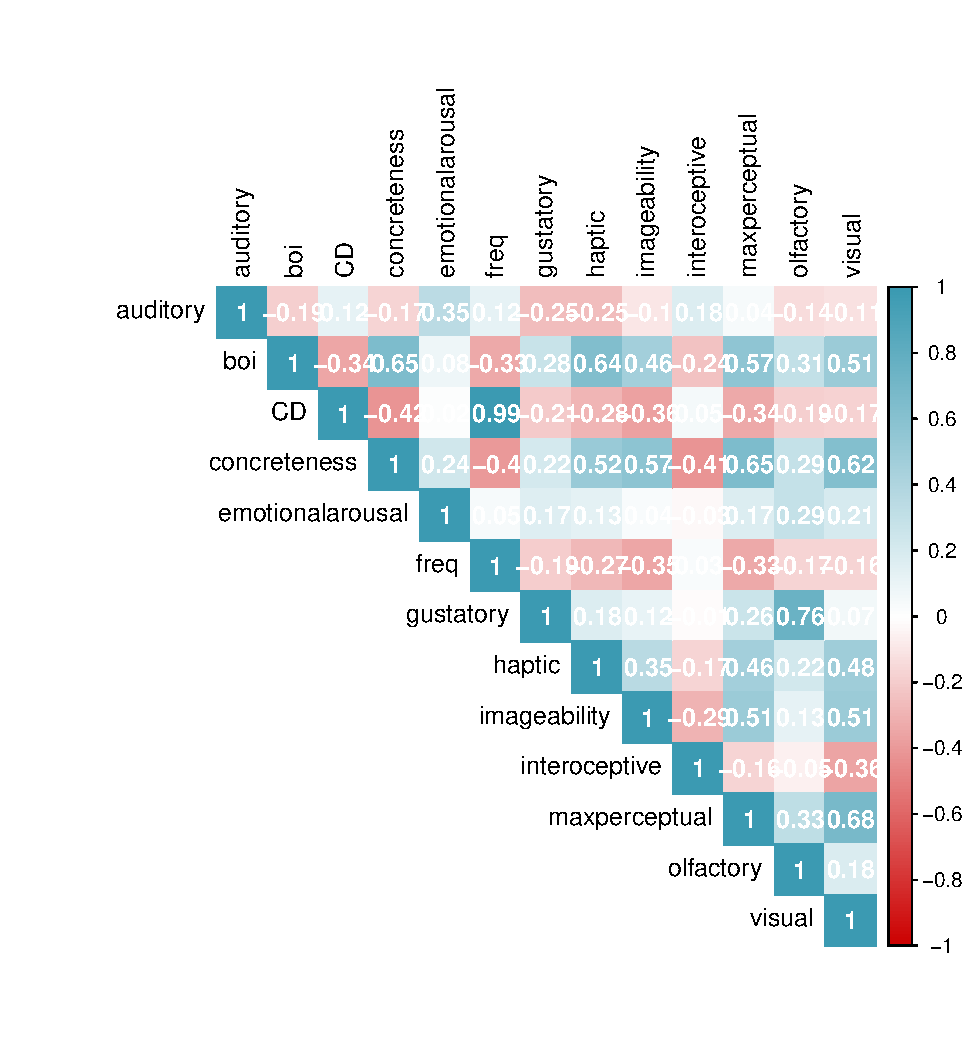
\includegraphics{crossling_abstractness_manuscript_files/figure-latex/variable-relationships-1.pdf}

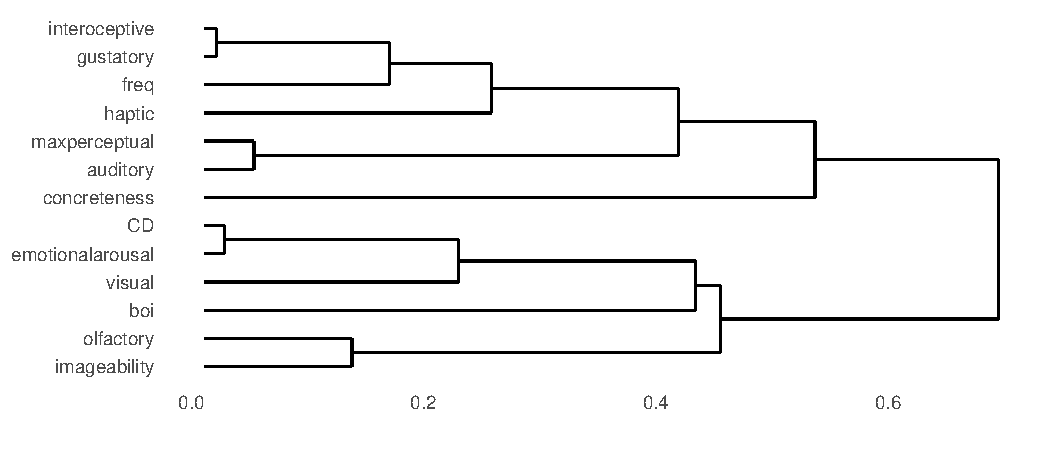
\includegraphics{crossling_abstractness_manuscript_files/figure-latex/variable-relationships-dendro-1.pdf}

\hypertarget{abstractness-effects-on-word-production}{%
\subsection{Abstractness effects on word production}\label{abstractness-effects-on-word-production}}

First, we fit a baseline statistical models for each language where word production is modeled as a combination of age, frequency, and phonological complexity. We then added each of our target predictors. For each target predictor for each language, it is thus possible to extract an effect size estimate of the target predictor and its interaction with age on the likelihood of word production. To explore heterogeneity and to estimate central tendency and variation in the effects, we borrow from meta-analytic techniques, treating each language as a study, and creating a weighted average of the effect size.

Figure \ref{fig:summary-of-maineffects} shows the coefficient estimate for each predictor in each language; see Table xxx for a full accounting of abstractness effect sizes. We find that iconicity is the strongest predictor of acquisition (mean across languages and measures: B = 0.12 (range: 0.07 - 0.35)). Many of the sensorimotor variables were relatively strong predictors of word production, including body-object-interaction (B = 0.1 (range: 0 - 0.4)), imageability (B = 0.1 (range: 0 - 0.21)), hapticness (B = 0.07 (range: -0.01 - 0.27)), and visualness (B = 0.05 (range: -0.05 - 0.17)). The effects of the social-emotional variables socialness (B = 0 (range: -0.2 - 0.15)) and emotional arousal ()--as well as several of the other sensorimotor variables (olfactoriness, interoceptiveness, auditoriness, and gustatoriness)--had much smaller mean effects on children's word production. Interestingly, concreteness was not reliably associated with word production across languages (B = -0.01 (range: -0.32 - 0.1)). Finally, the effect of context diversity was highly variable, with some languages showing large positive effects (e.g., ), while others showed large negative effects. Looking across languages, words which were used in more contexts were less likely to be produced (B = 0.01 (range: -0.21 - 0.14)).

\begin{figure}
\centering
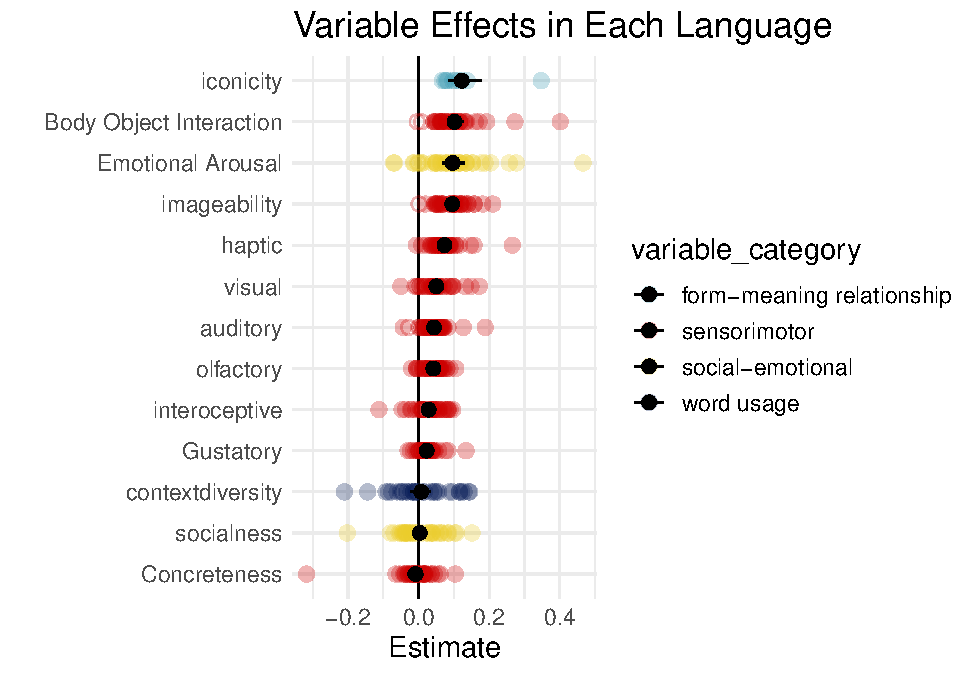
\includegraphics{crossling_abstractness_manuscript_files/figure-latex/summary-of-maineffects-1.pdf}
\caption{\label{fig:summary-of-maineffects}Effect size estimates (from logistic regression) of each of the abstractness variables studied. Each dot represents the effect size of one language, with filled-in dots showing significant effects and empty dots indicating that the effect was not significant in that language. Black dot and whiskers show mean effect size with standard error.}
\end{figure}

\hypertarget{developmental-change}{%
\subsubsection{Developmental Change}\label{developmental-change}}

Positive age interactions can be seen in at least xxx out of xxx languages for visualness, hapticness, body-object-interaction, and imageability. Conversely, there are negative age interactions for auditoryiness and iconicity in at least xxx out of xxx languages. This suggests that certain sensorimotor properties (chiefly, children's ability to see and touch a word's referent) facilitate learning more so later in development, while iconicity and auditoriness\footnote{The interaction between auditoriness and age was near 0 for both American Sign Language (B = xxx) and British Sign Language (B = xxx).} facilitate learning earlier in development. This result is consistent with the speculation above that xxx.

\begin{figure}
\centering
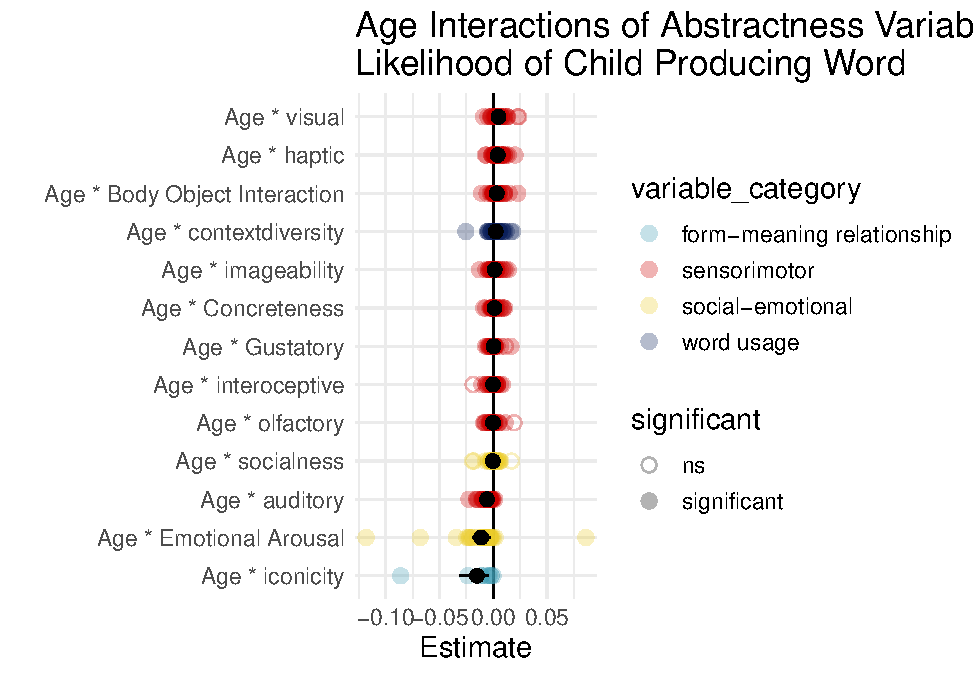
\includegraphics{crossling_abstractness_manuscript_files/figure-latex/summary-of-interactions-1.pdf}
\caption{\label{fig:summary-of-interactions}Effect size estimates (from logistic regression) of the interaction between each of the abstractness variables and age. Each dot represents the effect size of one language, with filled-in dots showing significant interactions and empty dots indicating that the effect was not significant in that language. Black dot and whiskers show mean effect size with standard error. Positive values show that effects are stronger for older children, while negative values show that effects are larger for younger children.}
\end{figure}

\hypertarget{what-drives-abstractness-effects}{%
\section{What drives abstractness effects?}\label{what-drives-abstractness-effects}}

Finally, we conduct an exploratory analysis aimed at measuring which of these abstractness variables best accounts for variability in words' production. Because these variables are interrelated, as shown in Figure xxx, when adding them to the same model, there is a risk of collinearity (Tomaschek et al., 2018). To get around this issue, we compare the predictive strength of the abstractness variables using random forest regression, implemented with the ranger package in R (Wright \& Ziegler, 2017). Random Forest regression is a machine learning method based on decision trees and recursive partitioning. Each tree is fit to a subset of the data and only uses a subset of the predictors (a third of the available variables in our analyses). The predictions of many hundreds of trees can then be averaged, which helps avoid overfitting and increases accuracy. Because Random Factor regression does not need to estimate a coefficient for every predictor variable in every tree, this approach allows us to avoid issues of collinearity, but the relative importance of two highly correlated predictors can still be compared by assessing the trees in which they do not co-occur.

This approach yields variance importance scores for each of the variables in our model. In Figure XXX, we display the overall ranking of the variance importance scores. We find that XXX is most important, followed by xxx.

Importance plots from random forest regression

We next explore the variability in ranking across languages. intra-class correlation of importance by variable across languages. we find an ICC of R = xxx, indicating xxx stability in relative importance of these predictors across languages.

\hypertarget{multiple-behavioral-tasks---abstractness-effects}{%
\subsection{Multiple behavioral tasks - abstractness effects}\label{multiple-behavioral-tasks---abstractness-effects}}

picture naming lexical decision

\hypertarget{discussion}{%
\section{Discussion}\label{discussion}}

Parents may not have an accurate sense of their children's comprehension of emotion words (\textbf{roepstorff2024?}).

\hypertarget{refs}{}
\begin{CSLReferences}{1}{0}
\leavevmode\vadjust pre{\hypertarget{ref-blomberg2015}{}}%
Blomberg, F., \& Öberg, C. (2015). Swedish and English word ratings of imageability, familiarity and age of acquisition are highly correlated. \emph{Nordic Journal of Linguistics}, \emph{38}(3), 351--364. \url{https://doi.org/10.1017/S0332586515000220}

\leavevmode\vadjust pre{\hypertarget{ref-bonin2018}{}}%
Bonin, P., Méot, A., \& Bugaiska, A. (2018). Concreteness norms for 1,659 {French} words: {Relationships} with other psycholinguistic variables and word recognition times. \emph{Behavior Research Methods}, \emph{50}(6), 2366--2387. \url{https://doi.org/10.3758/s13428-018-1014-y}

\leavevmode\vadjust pre{\hypertarget{ref-brysbaert2014}{}}%
Brysbaert, M., Warriner, A. B., \& Kuperman, V. (2014). Concreteness ratings for 40 thousand generally known {English} word lemmas. \emph{Behavior Research Methods}, \emph{46}(3), 904--911. \url{https://doi.org/10.3758/s13428-013-0403-5}

\leavevmode\vadjust pre{\hypertarget{ref-caselli2017a}{}}%
Caselli, N. K., Sehyr, Z. S., Cohen-Goldberg, A. M., \& Emmorey, K. (2017). {ASL-LEX}: {A} lexical database of {American Sign Language}. \emph{Behavior Research Methods}, \emph{49}(2), 784--801. \url{https://doi.org/10.3758/s13428-016-0742-0}

\leavevmode\vadjust pre{\hypertarget{ref-desrocher2009}{}}%
Desrocher. (2009). \emph{Subjective frequency and imageability ratings for 3,600 {French} nouns {\textbar} {SpringerLink}}.

\leavevmode\vadjust pre{\hypertarget{ref-diez-alamo2017}{}}%
Díez-Álamo, A. M., Díez, E., Alonso, M. A., Vargas, C. A., \& Fernandez, A. (2017). \emph{Normative ratings for perceptual and motor attributes of 750 object concepts in {Spanish}}.

\leavevmode\vadjust pre{\hypertarget{ref-hills2010}{}}%
Hills, T. T., Maouene, J., Riordan, B., \& Smith, L. B. (2010). The associative structure of language: {Contextual} diversity in early word learning. \emph{Journal of Memory and Language}, \emph{63}(3), 259--273. \url{https://doi.org/10.1016/j.jml.2010.06.002}

\leavevmode\vadjust pre{\hypertarget{ref-hills2009}{}}%
Hills, T. T., Maouene, M., Maouene, J., Sheya, A., \& Smith, L. (2009). Longitudinal {Analysis} of {Early Semantic Networks Preferential Attachment} or {Preferential Acquisition}? \emph{Psychological Science}, \emph{20}(6), 729--739. \url{https://doi.org/10.1111/j.1467-9280.2009.02365.x}

\leavevmode\vadjust pre{\hypertarget{ref-hinojosa2021}{}}%
Hinojosa, J. A., Haro, J., Magallares, S., Duñabeitia, J. A., \& Ferré, P. (2021). Iconicity ratings for 10,995 {Spanish} words and their relationship with psycholinguistic variables. \emph{Behavior Research Methods}, \emph{53}(3), 1262--1275. \url{https://doi.org/10.3758/s13428-020-01496-z}

\leavevmode\vadjust pre{\hypertarget{ref-hinojosa2020}{}}%
Hinojosa, José Antonio, Haro, J., Magallares, S., Ferré, P., \& Duñabeitia, J. A. (2020). \emph{Iconicity ratings for 10,995 {Spanish} words}. \url{https://doi.org/10.17605/OSF.IO/V5ER3}

\leavevmode\vadjust pre{\hypertarget{ref-jaruskova2023}{}}%
Jarůšková, L., Smolík, F., Chládková, K., Oceláková, Z., \& Paillereau, N. (2023). How to {Build} a {Communicative Development Inventory}: {Insights From} 43 {Adaptations}. \emph{Journal of Speech, Language, and Hearing Research}, \emph{66}(6), 2095--2117. \url{https://doi.org/10.1044/2023_JSLHR-22-00591}

\leavevmode\vadjust pre{\hypertarget{ref-kachergis2009}{}}%
Kachergis, G., Yu, C., \& Shiffrin, R. M. (2009). \emph{Frequency and {Contextual Diversity Effects} in {Cross-Situational Word Learning}}.

\leavevmode\vadjust pre{\hypertarget{ref-lynott2020}{}}%
Lynott, D., Connell, L., Brysbaert, M., Brand, J., \& Carney, J. (2020). The {Lancaster Sensorimotor Norms}: Multidimensional measures of perceptual and action strength for 40,000 {English} words. \emph{Behavior Research Methods}, \emph{52}(3), 1271--1291. \url{https://doi.org/10.3758/s13428-019-01316-z}

\leavevmode\vadjust pre{\hypertarget{ref-miceli2021}{}}%
Miceli, A., Wauthia, E., Lefebvre, L., Ris, L., \& Simoes Loureiro, I. (2021). Perceptual and {Interoceptive Strength Norms} for 270 {French Words}. \emph{Frontiers in Psychology}, \emph{12}, 667271. \url{https://doi.org/10.3389/fpsyg.2021.667271}

\leavevmode\vadjust pre{\hypertarget{ref-miklashevsky2018}{}}%
Miklashevsky, A. (2018). Perceptual {Experience Norms} for 506 {Russian Nouns}: {Modality Rating}, {Spatial Localization}, {Manipulability}, {Imageability} and {Other Variables}. \emph{Journal of Psycholinguistic Research}, \emph{47}, 641--661. \url{https://doi.org/10.1007/s10936-017-9548-1}

\leavevmode\vadjust pre{\hypertarget{ref-muraki2022}{}}%
Muraki, E. J., Siddiqui, I. A., \& Pexman, P. M. (2022). Quantifying children's sensorimotor experience: {Child} body-object interaction ratings for 3359 {English} words. \emph{Behavior Research Methods}, \emph{54}(6), 2864--2877. \url{https://doi.org/10.3758/s13428-022-01798-4}

\leavevmode\vadjust pre{\hypertarget{ref-rofes2018}{}}%
Rofes, A., Zakariás, L., Ceder, K., Lind, M., Johansson, M. B., de Aguiar, V., \ldots{} Howard, D. (2018). Imageability ratings across languages. \emph{Behavior Research Methods}, \emph{50}(3), 1187--1197. \url{https://doi.org/10.3758/s13428-017-0936-0}

\leavevmode\vadjust pre{\hypertarget{ref-rosa2022}{}}%
Rosa, E., Salom, R., \& Perea, M. (2022). Contextual diversity favors the learning of new words in children regardless of their comprehension skills. \emph{Journal of Experimental Child Psychology}, \emph{214}, 105312. \url{https://doi.org/10.1016/j.jecp.2021.105312}

\leavevmode\vadjust pre{\hypertarget{ref-sehyr2021}{}}%
Sehyr, Z. S., Caselli, N. K., Cohen-Goldberg, A. M., \& Emmorey, K. (2021). The {ASL-LEX} 2.0 {Project}: {A Database} of {Lexical} and {Phonological Properties} for 2,723 {Signs} in {American Sign Language}. \emph{The Journal of Deaf Studies and Deaf Education}, \emph{26}(2), 263--277. \url{https://doi.org/10.1093/deafed/enaa038}

\leavevmode\vadjust pre{\hypertarget{ref-seidl2023}{}}%
Seidl, A. H., Indarjit, M., \& Borovsky, A. (2023). Touch to learn: {Multisensory} input supports word learning and processing. \emph{Developmental Science}. \url{https://doi.org/10.1111/desc.13419}

\leavevmode\vadjust pre{\hypertarget{ref-soares2017}{}}%
Soares, A. P., Costa, A. S., Machado, J., Comesana, M., \& Oliveira, H. M. (2017). The {Minho Word Pool}: {Norms} for imageability, concreteness, and subjective frequency for 3,800 {Portuguese} words {\textbar} {SpringerLink}. \emph{Behavior Research Methods}, \emph{49}, 1065--1081. \url{https://doi.org/10.3758/s13428-016-0767-4}

\leavevmode\vadjust pre{\hypertarget{ref-speed2022}{}}%
Speed, L. J., \& Brybaert, M. (2022). Dutch sensory modality norms. \emph{Behavior Research Methods}, \emph{54}(3), 1306--1318. \url{https://doi.org/10.3758/s13428-021-01656-9}

\leavevmode\vadjust pre{\hypertarget{ref-torkamani-azar2019}{}}%
Torkamani-Azar, M., Kanik, S. D., Vardan, A. T., Aydin, C., \& Cetin, M. (2019). Emotionality of {Turkish} language and primary adaptation of affective {English} norms for {Turkish}. \emph{Current Psychology}, \emph{38}(2), 273--294. \url{https://doi.org/10.1007/s12144-018-0119-x}

\leavevmode\vadjust pre{\hypertarget{ref-vergallito2020}{}}%
Vergallito, A., Petilli, M. A., \& Marelli, M. (2020). Perceptual modality norms for 1,121 {Italian} words: {A} comparison with concreteness and imageability scores and an analysis of their impact in word processing tasks. \emph{Behavior Research Methods}, \emph{52}(4), 1599--1616. \url{https://doi.org/10.3758/s13428-019-01337-8}

\leavevmode\vadjust pre{\hypertarget{ref-verheyen2020}{}}%
Verheyen, S., De Deyne, S., Linsen, S., \& Storms, G. (2020). Lexicosemantic, affective, and distributional norms for 1,000 {Dutch} adjectives. \emph{Behavior Research Methods}, \emph{52}(3), 1108--1121. \url{https://doi.org/10.3758/s13428-019-01303-4}

\leavevmode\vadjust pre{\hypertarget{ref-winter2023a}{}}%
Winter, B., Lupyan, G., Perry, L. K., Dingemanse, M., \& Perlman, M. (2023). Iconicity ratings for 14,000+ {English} words. \emph{Behavior Research Methods}. \url{https://doi.org/10.3758/s13428-023-02112-6}

\leavevmode\vadjust pre{\hypertarget{ref-zhong2022}{}}%
Zhong, Y., Wan, M., Ahrens, K., \& Huang, C.-R. (2022). Sensorimotor norms for {Chinese} nouns and their relationship with orthographic and semantic variables. \emph{Language, Cognition and Neuroscience}, \emph{37}, 1--23. \url{https://doi.org/10.1080/23273798.2022.2035416}

\end{CSLReferences}


\end{document}
